
\documentclass{tufte-book}
\usepackage{titling}
\usepackage{fancyhdr}
\pagestyle{fancy}
\fancyhf{}
\rhead{\thesection}
\lhead{}
\rfoot{\color{titlecolor}{ Page \thepage}}
\usepackage[parfill]{parskip}
\usepackage{verbatim}
\usepackage{mystyle}
\usepackage{natbib}
\usepackage{amsmath}
\usepackage{longtable}
\everymath{\displaystyle}
\providecommand{\tightlist}{%
  \setlength{\itemsep}{0pt}\setlength{\parskip}{0pt}}
\begin{document}
\hypertarget{macro-economics}{%
\section{Macro Economics}\label{macro-economics}}

\hypertarget{gdp}{%
\subsection{GDP}\label{gdp}}

\begin{description}
\item[GDP(Gross Domestic product)]
The Total amount of goods and services produced within an economy in a
given year \footnote{There are three ways of culculating this

  \begin{itemize}
  \item
    Expenditure : This must only include expenditure on goods and
    services produced within the economy (no imports, and no goods
    produced in a previous year)
  \item
    Income : This must only use income obtained by selling goods and
    services (no transfer payments)
  \item
    Output
  \end{itemize}}
\end{description}

\hypertarget{gdp-composition}{%
\section{GDP composition}\label{gdp-composition}}

To measure the GDP\footnote{GDP and total demand(Z) are used
  interchangably} it is simplest to measure the amount spent on goods
and services and then subtract the part of that which is spent on goods
and services produced outside the economy (imports) or before the given
year (invetories). Finaly goods not bought in the bought elsewhere
(exports) or stored for the future are added.\footnote{Exports and
  inventories are ignored in the begining part of the course}

\begin{itemize}
\tightlist
\item
  Consumption(C): The goods and services purchased by consumers
\item
  Investment(I): The sum of

  \begin{itemize}
  \tightlist
  \item
    no-resedential investment: Capital equipment and land bought by
    firms
  \item
    resedntial investment: Housing bought by consumers
  \end{itemize}
\item
  Goverment spending(G): The amount the goverment spendings buying goods
  and services from firms and employing workers. (goverment tranfers are
  not payments for work done and are not included)
\item
  Net exports (X-I): The total amount of exports minus imports.
\item
  Net inventory build up
\end{itemize}

This brings us to the equation \(Z = C + I + G\)

\hypertarget{consumption}{%
\subsection{Consumption}\label{consumption}}

Consumption is a function of disposable income \footnote{income minus
  taxation} (\(Y_D\)) \[ C(Y_D) \]

\hypertarget{unemployment}{%
\subsection{Unemployment}\label{unemployment}}

\hypertarget{inflation}{%
\subsection{Inflation}\label{inflation}}

\hypertarget{philips-curve}{%
\subsection{Philips curve}\label{philips-curve}}\hypertarget{islm-model}{%
\section{ISLM model}\label{islm-model}}

The ISLM model models the equilibrium for income and interest rates, the
quintity of money supplied and consumption.

This is represented by the intersenctoin of the IS curve which shows the
resultant intrest rates for all equilibriums between money demand which
is a function of income and money supply, and the LM curve which
represents all the points of equilibrium (where consumption is equil to
output and no inventories are built up or depleted) and consuption
(which contains investment which is a function of interest rates)

\hypertarget{first-model}{%
\subsection{First model}\label{first-model}}

\begin{quote}
** Assumption ** The economy is closed and there is no public
sector(taxation or gorverment spending)
\end{quote}

\begin{figure}
\centering
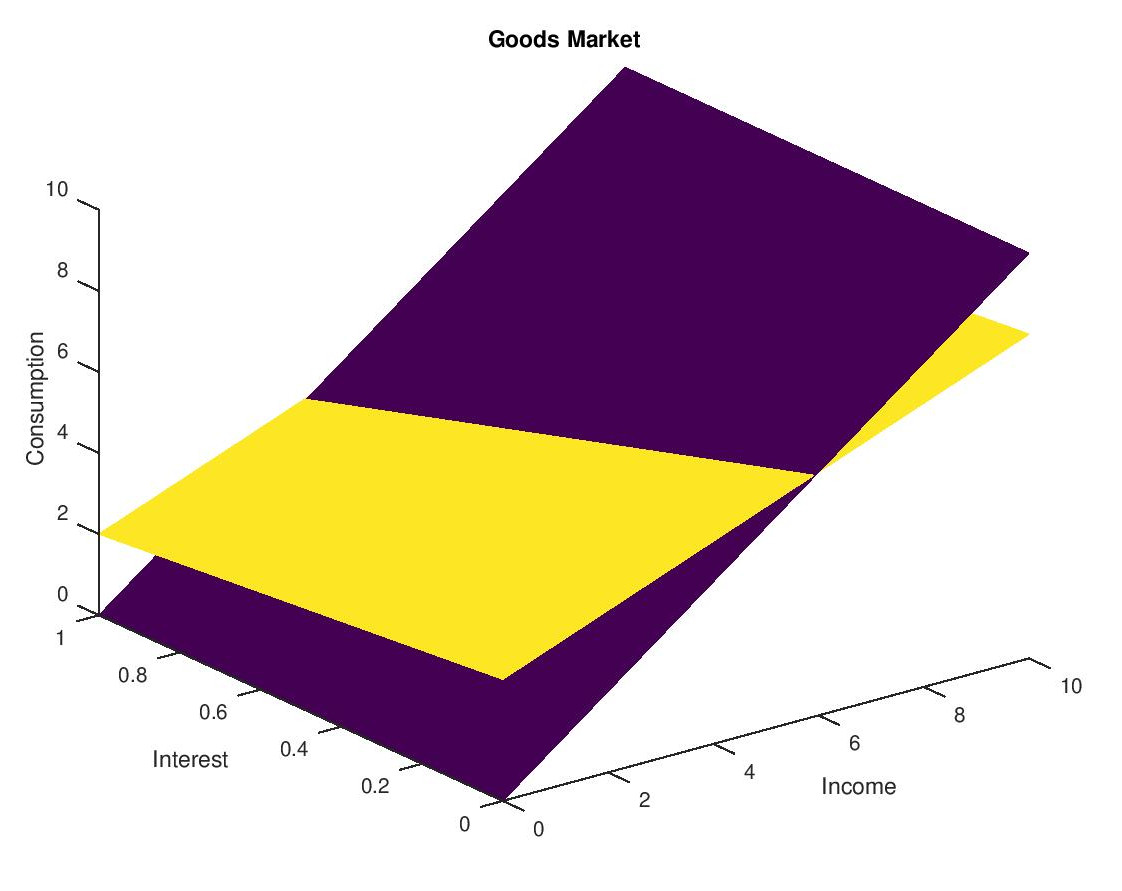
\includegraphics[width=\textwidth,height=1\textwidth]{pics/LM.jpg}
\caption{IS}
\end{figure}

\hypertarget{the-is-curve-give-all-points-of-equilibrium-in-the-financial-market}{%
\subsection{The IS curve give all points of equilibrium in the financial
market}\label{the-is-curve-give-all-points-of-equilibrium-in-the-financial-market}}

\begin{figure}
\centering
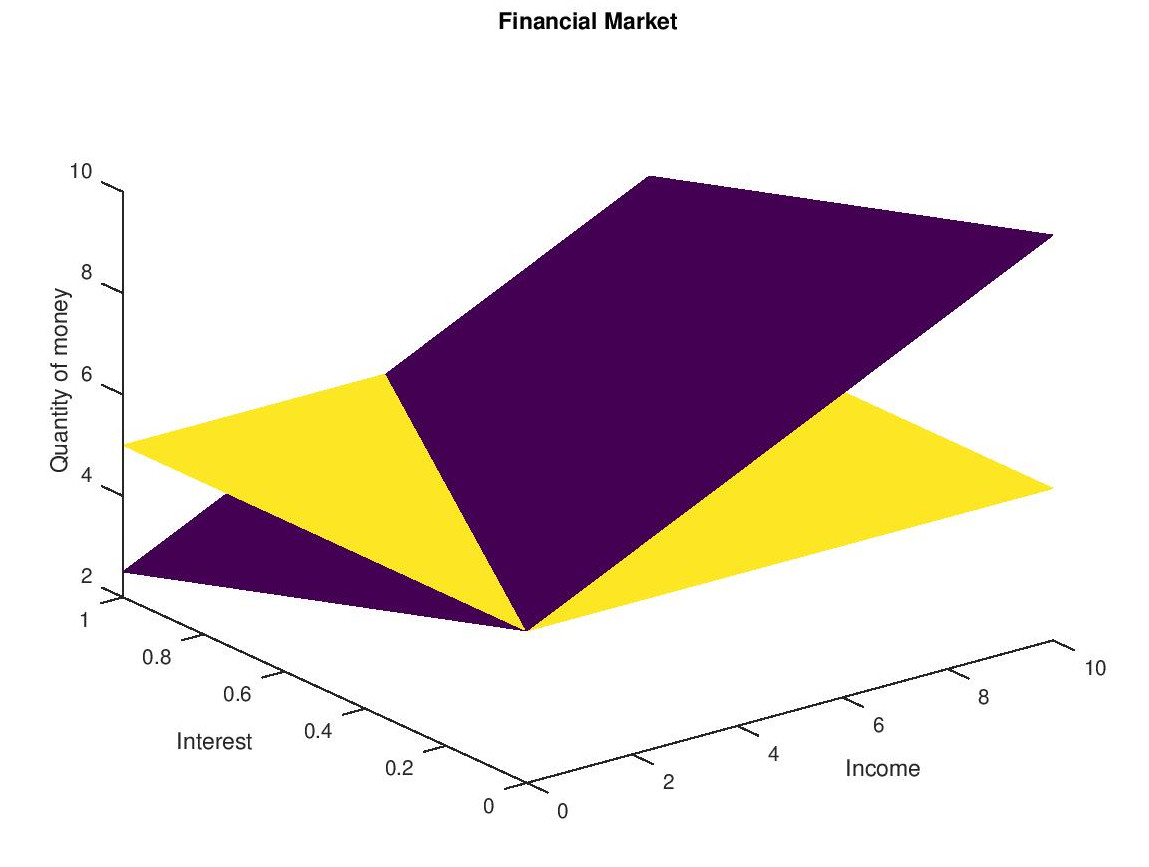
\includegraphics[width=\textwidth,height=1\textwidth]{pics/IS.jpg}
\caption{LM}
\end{figure}\hypertarget{financial-markets}{%
\section{Financial Markets}\label{financial-markets}}

\hypertarget{the-demand-for-money}{%
\subsection{The Demand for money}\label{the-demand-for-money}}

Is the demand for liquidity and comes from people wanting to make
purchases with that money.

\hypertarget{supply-of-money}{%
\subsection{Supply of money}\label{supply-of-money}}

The supply of money is modeled as a constant \(M\) and supplied by the
centerall bank

\hypertarget{monatary-policy-and-open-market-operations-58}{%
\subsection{Monatary policy and open market operations
58}\label{monatary-policy-and-open-market-operations-58}}\hypertarget{bonds}{%
\section{Bonds}\label{bonds}}

Bonds have

\begin{itemize}
\tightlist
\item
  \(P\) a face value that they are sold and rebought by the issuer
\item
  \(i\) an interest rate paid repesenting the charge per unit currency
  borrowed paid by the bonds issueur to the bonds owner.
\end{itemize}

In the market for bonds

\begin{itemize}
\tightlist
\item
  \(i_e\) is the equilibrium interest rate for bonds of a ccertain risk.
\end{itemize}

No bonds will be bought by from sellers selling assets yeilding bellow
this interest rate.

This means that the asset must be sold at a maket price \(P_m\) such
that the interest it yeilds \(Pi\) is the equilibrium rate of interest
\(i_e\)

\(\frac{Pi}{P_m} = i_e\)

This give a counterintuitive result that the market prce and the market
interest rates are inversly related. If the interest rate on a bond has
increased this would seem to make it more disarable and so increase its
prices, but this is not what has happened. Other bonds of similar risk
are being sold on the market at higher interest rates, (Or lower costs
and set interet) while the bond retains the same interst.\hypertarget{macro-economic-terms}{%
\section{Macro Economic Terms}\label{macro-economic-terms}}

\begin{description}
\tightlist
\item[GDP]
A monatary measure of the total market value of final goods and services
produced in a country in a given period of time.
\end{description}

\textbf{VAT is included in GDP as a cost of production?} This can be
calculated in three ways

\begin{verbatim}
* Income to all factors of production for produceing the goods and services
    + Compensation for employees
    + Rent
    + Interest
    + Proprietors income (unincorporated busnessess)
    + Corporate Profits
      - Corporate income taxes ? why not add taxes in general rather than just not deduct them?
      - dividends
      - retained profits
* Output (Value added) measured as value added at all levels of production
* Expenditure on final goods and services produced within a country ^[eports - imports]
  Also includes investment in new capitial equipment and real estate a minus depreciation^[Where is depreciation accounted fro in the other two apporchers?]

     This is the same as the expenditure or damand function function

      +  $E = C + I + G +(X - M)$
\end{verbatim}

\begin{quote}
GDP Excludes

\begin{itemize}
\tightlist
\item
  Public transfer payments
\item
  Private Trasnfer payments
\item
  Sales of stocks and bonds
\item
  Second hand sales
\end{itemize}
\end{quote}

\begin{description}
\tightlist
\item[NI]
All income earned by domestic-supplied resouces. (Those owned by
citizens?)
\end{description}

Calculating NI from GDP

\begin{itemize}
\item
  Subtract Vat from GDP
\item
\end{itemize}

\begin{description}
\tightlist
\item[GNP]
The total value of goods and services produced by a countries citizens
within a given period of time.
\item[Real GDP]
Inflation adjusted GDP
\item[Nominal GDP]
GDP measured in the market prices of the current year.
\item[NDP]
Includes factor depreciation
\end{description}\end{document}